\chapter{Конструкторский раздел}
\label{cha:design}

В данном разделе рассматриваются реализуемые алгоритмы и методы, приводятся выкладки по модификации существующих.

\section{Генерация мгновенного снимка и подготовка буферов для работы методов размытия движения}

\subsection{Нахождение точек полигона}

Любой выпуклый полигон можно представить в виде пересекающихся прямых. Точки пересечения данных прямых будут являются вершинами выпуклого многоугольника. Каждый пиксель данного многоугольника можно найти, при его сканировании сверху вниз. Необходимо найти абсциссы пересечений сканирующей строки и граней. Чтобы определить с какими гранями нужно искать пересечение, достаточно сравнить ординату сканирующей строки и ординаты точек отрезков: $P_{1y} \leq y \leq P_{2y}$, причем $P_{1y} \leq P_{2y}$. Ребра, удовлетворяющие данному условию, будем называть активными. Для горизонтальных ребер пересечений со сканирующей строкой не нужно.

Необходимо заметить, что для выпуклого многоугольника сканирующая строка всегда пересекает ровно два ребра, т.е. существует только два активных ребра. Следовательно, можно заранее сформировать массив ребер и отсортировать его по координатам $y,x$ вершине ребра с наибольшим значением $y$. 

Для упрощения нахождения пересечений отрезков со сканирующей строкой можно искать значения прямых пошагово. Если задать уравнение прямой формулой $x(y) = ky + m$, то $\frac{\delta x}{\delta y} = k = \frac{P_{1x} - P_{2x}}{P_{1y} - P_{2y}}$. Следовательно $x(y + 1) = x(y) + k$. Т.к. горизонтальные ребра были исключены из рассмотрения, значит $k \neq \pm \infty$. Представим операцию подготовки массива ребер с помощью псевдокода \ref{alg:A_MakeEdges}.

\begin{breakablealgorithm}
    \caption{Подготовка массива ребер}\label{alg:A_MakeEdges}
    
    \begin{algorithmic}[1]
    \Function{MakeEdges}{points}
        \Statex $\triangleright$ $points$ "--- вершины полигона 
        \Statex
        \State $edges \leftarrow$ пустой массив ребер      
        \State $count \leftarrow $ длина массива $points$
        \State $temp \leftarrow$ пустое ребро
        \ForAll{$i \in [0; count]$}
            \State $temp.begin \leftarrow points[i]$
            \State $temp.end \leftarrow points[(i+1)\mod count]$
            \If{ребро $temp$ не горизонтальное}
                \If{$temp.begin.y > temp.end.y$}
                    \State $temp \leftarrow (temp[1], temp[0])$
                \EndIf
    
                \State $temp.k \leftarrow \frac{temp.begin.x - temp.end.x}{temp.begin.y - temp.end.y}$
                \State Добавить $temp$ в массив $edges$
            \EndIf
        \EndFor
        
        \State отсортировать массив $edges$ по координатам $y$ и $x$ первой вершины ребра
    
        \State \Return $edges$
    
    \EndFunction
    \end{algorithmic}
\end{breakablealgorithm}

Далее из данного массива необходимо получать активные ребра по мере просмотра многоугольник сверху вниз. 



Для правильной работы алгоритма удаления невидимых линий и поверхностей, также для каждой точки полигона необходимо найти координату $z$. Её можно получить из уравнения плоскости: $Ax + By + Cz + D = 0$, которое находится по трем точкам, не лежащих на одной прямой.

Путь $P_1$, $P_2$, $P_3$ - вершины полигона, не лежащие на одной прямой, тогда найдем два вектора, определяющих плоскость полигона: $\vec{a} = P_1 - P_2 $, $\vec{b} = P_1 - P_3 $. Из свойств векторного произведения: векторное произведение $\vec{a} \times \vec{b}$  есть нормаль к плоскости, образованной векторами $\vec{a}$ и $\vec{b}$. Также известно, что коэффициенты $A$, $B$, $C$  в уравнение плоскости задают нормаль к данной плоскости $ \vec{n} = \begin{pmatrix}
        A & B & C
    \end{pmatrix}$. Векторное произведение можно найти по формуле \eqref{F:vector_scalar}.

\begin{equation}
    \label{F:vector_scalar}
    \vec{n} = \vec{a} \times \vec{b} = \begin{pmatrix}
        \vec{a}_y \vec{b}_z - \vec{a}_z \vec{b}_y &
        \vec{a}_z \vec{b}_x - \vec{a}_x \vec{b}_z &
        \vec{a}_x \vec{b}_y - \vec{a}_y \vec{b}_x
    \end{pmatrix}
\end{equation}

Оставшийся коэффициент $D$ находим, подставляя произвольную точку плоскости в уравнение данной плоскости. С учетом данного факта получим уравнение функции \eqref{F:F_ploskost_koef} нахождения коэффициентов плоскости по точке данной плоскости и двух векторов, лежащих в этой плоскости.


\begin{equation}
    \label{F:F_ploskost_koef}
    FindSurf(P, \vec{a}, \vec{b}) =
    \begin{pmatrix}
        A \\
        B \\
        C \\
        D
    \end{pmatrix} =
    \begin{pmatrix}
        \vec{a}_y \vec{b}_z - \vec{a}_z \vec{b}_y \\
        \vec{a}_z \vec{b}_x - \vec{a}_x \vec{b}_z \\
        \vec{a}_x \vec{b}_y - \vec{a}_y \vec{b}_x \\
        -A \cdot P_x - B \cdot P_y - C \cdot P_z
    \end{pmatrix}
\end{equation}

Зная точки $x$, $y$ полигона и коэффициенты плоскости можно найти координату $z$. Обозначим данную функцию как $FindZ(surf, point)$, представленную на формуле \eqref{F:F_FindZ}.

\begin{equation}
    \label{F:F_FindZ}
    FindZ(surf, point) = -\frac{surf_A \cdot point_x + surf_B \cdot point_y + surf_D}{surf_C}
\end{equation}

Для упрощения процесса нахождения координаты $z$ во время прохода по сканирующей строке можно считать значение пошагово по формуле \eqref{F:F_z_iterative_find_depth}.

\begin{eqndesc}
    \begin{equation}
        \label{F:F_z_iterative_find_depth}
        FindNextZ(k, z) = FindZ(surf, point)  + \frac{\delta (FindZ(surf, point))}{\delta x} =
        z + k
    \end{equation}
    , где
    $k = \frac{A}{C}$ "--- приращение $z$ для плоскости $surf$
\end{eqndesc}

\subsection{Нахождение вектора скорости пикселя}

Для работы методов размытия необходим буфер скоростей пикселей. Заметим, что скорость $v = \begin{pmatrix}
        {\Delta x} & {\Delta y}
    \end{pmatrix}$ пикселя задается в плоскости изображения, т.е. с учетом преобразований камеры.

Так как любое перемещение объекта задается изменением положения, поворота и масштаба тела относительно его центра, то данное перемещение можно представить с помощью последовательного произведения матриц преобразования, указанных в таблице \ref{tab:tranformations_table}. Данную матрицу будем задавать как $Transf(c, \vec{t}, \vec{k}, \vec{r})$, где $c$ "--- центр тела, $\vec{t}$ "--- перемещение тела, $\vec{k}$ "--- увеличение тела, $r$ "--- поворот тела. Вектора указаны в системе координат сцены.
\begin{center}
    \begin{longtable}{|p{0.115\textwidth}|p{0.41\textwidth}|p{0.43\textwidth}|}
        \caption{Необходимые преобразования и порядок их применения}
        \label{tab:tranformations_table}
        \\ \hline
        № применения & Матрица преобразования                    & Описание преобразования                                                    \\
        \hline \endfirsthead
        \subcaption{Продолжение таблицы~\ref{tab:tranformations_table}}
        \\ \hline \endhead
        \hline \subcaption{Продолжение на след. стр.}
        \endfoot
        \hline \endlastfoot
        1            & $
            \begin{pmatrix}
                1   & 0   & 0   & 0 \\
                0   & 1   & 0   & 0 \\
                0   & 0   & 1   & 0 \\
                c_x & c_y & c_z & 1 \\
            \end{pmatrix}
        $            & Перенос начала координат в центр тела $c$                                                                              \\
        \hline
        2            & $\begin{pmatrix}
                1 & 0              & 0               & 0 \\
                0 & \cos(\alpha_x) & -\sin(\alpha_x) & 0 \\
                0 & \sin(\alpha_x) & \cos(\alpha_x)  & 0 \\
                0 & 0              & 0               & 1 \\
            \end{pmatrix}$               & Поворот тела вдоль оси $x$ на угол $\alpha_x$                              \\
        \hline
        3            & $\begin{pmatrix}
                \cos(\alpha_y) & 0 & -\sin(\alpha_y) & 0 \\
                0              & 1 & 0               & 0 \\
                \sin(\alpha_y) & 0 & \cos(\alpha_y)  & 0 \\
                0              & 0 & 0               & 1 \\
            \end{pmatrix}$              & Поворот тела вдоль оси $y$ на угол $\alpha_y$                              \\
        \hline
        4            & $\begin{pmatrix}
                \cos(\alpha_z) & -\sin(\alpha_z) & 0 & 0 \\
                \sin(\alpha_z) & \cos(\alpha_z)  & 0 & 0 \\
                0              & 0               & 0 & 1 \\
                0              & 0               & 1 & 0
            \end{pmatrix}$              & Поворот тела вдоль оси $z$ на угол $\alpha_z$                              \\
        \hline
        5            & $\begin{pmatrix}
                k_x & 0   & 0   & 0 \\
                0   & k_y & 0   & 0 \\
                0   & 0   & k_z & 0 \\
                0   & 0   & 0   & 1 \\
            \end{pmatrix}$              & Выполнение масштабирования тела на $k_x$, $k_y$, $k_z$                     \\
        \hline
        6            & $\begin{pmatrix}
                1        & 0        & 0        & 0 \\
                0        & 1        & 0        & 0 \\
                0        & 0        & 1        & 0 \\
                dx - c_x & dy - c_y & dz - c_z & 1
            \end{pmatrix}$              & Выполнение перемещения тела на $dx$, $dy$, $dz$ и возврат начала координат \\


        \hline
    \end{longtable}
\end{center}
Для более структурированного повествования для каждого тела $object$, введем их параметры в виде функций, зависящих от времени:
\begin{itemize}
    \item $object.pos(t)$ "--- положение центра тела в момент времени $t$;
    \item $object.rot(t)$ "--- поворот тела относительно центра в момент $t$;
    \item $object.scale(t)$ "--- масштаб тела относительно центра в момент $t$.
\end{itemize}

Следовательно, зная масштаб $object.scale$, положение $object.pos$, поворот $object.rot$ некоторого тела $object$ в моменты времени $t_0$ и $t_1$, где время выдержки $\Delta T = t_1 - t_0 > 0$, можно найти положения вокселя $p = (x,y,z)$ в координатах сцены через $\Delta T$ с помощью матрицы преобразования, представленной на формуле \eqref{F:F_ObjectMatrix}.


\begin{equation}
    \label{F:F_ObjectMatrix}
    \begin{matrix}
        {
            ObjectMatrix(object, t, \Delta T) =
            Transf(
            object.pos(t),
        } \\

        {
        object.pos(t + \Delta T) - object.pos(t),

        }
        {\frac{object.scale(t + \Delta T)}{object.scale(t)}, }\\{  object.rot(t + \Delta T) - object.rot(t))}
    \end{matrix}
\end{equation}


Чтобы перейти в координаты сцены из системы координат изображения, необходимо умножить координаты вокселя $p$ на обратную матрицу преобразования камеры $(Cam(cam, t_0))^{-1} = ICam(cam, t_0)$ в момент времени $t_0$. Чтобы вернуться в систему координат изображения, необходимо домножить на матрицу преобразования камеры $Cam(cam, t_0 + \Delta T)$ в момент времени $t_0 + \Delta T$.

Тогда можем получить координаты вокселя $p_1$ в пространстве изображения через время выдержки $\Delta T$. Запишем преобразования \eqref{F:F_voxel_transf} нахождения положения вокселя $p$ через время выдержки $\Delta T$ какого-то тела.

\begin{equation}
    \label{F:F_voxel_transf}
    \begin{matrix}
        {VoxelTransf(Cam, ICam, ObjectMatrix) =} \\
        {= ICam(cam, t_0) \times ObjectMatrix(object, t, \Delta T) \times Cam(cam, t_0 + \Delta T)}
    \end{matrix}
\end{equation}

Зная положения вокселя $p$ в моменты времени начала и окончания выдержки возможно найти скорость пикселя по формуле \eqref{F:F_voxel_speed}.

\begin{eqndesc}
    \begin{equation}
        \label{F:F_voxel_speed}
        FindV(p_0, VoxelTransf) = p_0 - p_0 \times VoxelTransf(Cam, ICam, ObjectMatrix)
    \end{equation}
\end{eqndesc}
\subsection{Учет положения и угла поворота камеры}
В предыдущем пункте было упомянуто о матрице преобразования камеры $Cam(cam, t)$, вывод которой будет рассмотрен в данном пункте.

Камера $cam$ также является объектом, но кроме параметров, приведенных в предыдущем пункте, также содержит коэффициент перспективы $cam.k$.

Можно задать преобразование, которое перемещает систему координат сцены в систему координат камеры, через матрицу $Cam(t)$, заданную формулой \eqref{F:F_Cam_Matrix}.

\begin{eqndesc}
    \begin{equation}
        \label{F:F_Cam_Matrix}
        \begin{matrix}
            {Cam(cam, t) = Transf(cam.pos(t), -cam.pos(t),} \\{ cam.scale(t), cam.rot(t)) \times Persp(k)}
        \end{matrix}
    \end{equation}
    , где
    $Persp(k)$ "--- перспективное преобразование, заданное формулой \eqref{F:F_persp_matrix}\\
\end{eqndesc}

\begin{equation}
    \label{F:F_persp_matrix}
    Persp(k) = \begin{pmatrix}
        1 & 0 & 0 & 0 \\
        0 & 1 & 0 & 0 \\
        0 & 0 & 1 & k \\
        0 & 0 & 0 & 1 \\
    \end{pmatrix}
\end{equation}

Также для вычислений необходима обратная матрица преобразования камеры $(Cam(cam, t))^{-1}$. Её можно задать формулой \eqref{F:F_inv_cam_matrix}

\begin{equation}
    \label{F:F_inv_cam_matrix}
    \begin{matrix}
        {ICam(cam, t) = (Cam(cam, t))^{-1} = Persp(-k) \times} \\
        {\times Transf(\vec{0}, cam.pos(t), \frac{1}{cam.scale(t)}, -cam.rot(t))}
    \end{matrix}
\end{equation}

\subsection{Модификация алгоритма построения изображения с помощью z-буфера}


Данный алгоритм для каждого кадра буфер изображения $V$ заполняет цветом фона, буфер глубины $Z$ - максимальной величиной (бесконечностью), буфер скоростей пикселей $v$ зануляет. 

Алгоритм подразумевает предварительное формирование матрицы преобразования камеры $CamM = Cam(cam, t)$ и обратной матрицы $ICamM = ICam(cam, t + \Delta T)$, чтобы производить вычисления в пространстве объектов. Также для каждой модели $model$ необходимо преобразование вокселя $VoxelTransf(Cam, ICam, ObjectMatrix(model, t, \Delta T))$.  

Для отрисовки единичного полигона представлен псевдокод \ref{alg:A_DrawPolygon}.  На вход данной функции поступают $p$ "--- вершины полигона, $color$ "--- цвет полигона, $V$, $z$, $v$ "--- буферы кадра, глубины и скорости соответственно и матрица преобразования вокселя $VoxelTransfM$.


\begin{breakablealgorithm}
\caption{Модифицированный алгоритм удаления невидимых линий и поверхностей с помощью z-буфера и формирования буфера скоростей} \label{alg:A_DrawPolygon}

\begin{algorithmic}[1]
\Function{DrawPolygon}{$V, Z, v, p, color, VoxelTransfM$}
    \State 
        $surf \leftarrow FindSurf(
            p[0],
            p[0] - p[1],
            p[0] - p[2]
        )$
        \Comment коэффициенты плоскости полигона для поиска глубины
    \State $kz \leftarrow \frac{surf.A}{surf.C}$    
    \Statex

    \State $edges \leftarrow MakeEdges(p)$ \Comment см. псевдокод \ref{alg:A_MakeEdges} 
    
    \State $edgeL \leftarrow edges[0]$ 
    \State $edgeR \leftarrow edges[1]$
    \State $last \leftarrow 1$ 
    \Statex
    \State $xL \leftarrow edgeL.begin.x$ 
    \State $xR \leftarrow edgeR.begin.x$

    \Statex \Comment т.к. массив ребер отсортирован, то в силу выпуклости полигона получим минимальное и максимальное значения $y$
    \State $y_{min} \leftarrow edges[0].begin.y$
    \State $y_{max} \leftarrow edges[$ последний элемент $].end.y$ 

    \ForAll{$y \in [y_{min}, y_{max}]$} 
        
        \State $z \leftarrow FindZ(x,y, surf)$ \Comment см. формулу \eqref{F:F_FindZ} 
        \ForAll{$x \in [xL, xR]$} 
            \If{$z < Z[x,y]$}
                \State $V[x,y] \leftarrow color$
                \State $Z[x,y] \leftarrow z$
                \State $v[x,y] \leftarrow FindV((x,y,z,1), VoxelTransfM)$ 
                \Statex \Comment см. формулу \eqref{F:F_voxel_speed} 
            \EndIf
            \State $z \leftarrow FindNextZ(kz, z)$ \Comment см. формулу \eqref{F:F_z_iterative_find_depth} 
        \EndFor
        \State $xL \leftarrow xL + kL$
        \State $xR \leftarrow xR + kR$
        \If{$edgeL.end.y \leq y$}
            \State $last \leftarrow last + 1$
            \State $edgeL \leftarrow edges[last]$
            \State $xL \leftarrow edgeL.begin.x$ 
        \EndIf
        
        \If{$edgeR.end.y \leq y$}
            \State $last \leftarrow last + 1$
            \State $edgeR \leftarrow edges[last]$
            \State $xR \leftarrow edgeR.begin.x$ 
        \EndIf

    \EndFor
    
\EndFunction
\Statex 

\end{algorithmic}
\end{breakablealgorithm}

Для получения финального мгновенного кадра с решением проблемы удаления невидимых линий и поверхностей, а также поиска буферов глубины и скоростей необходимо данную операцию применить для каждого полигона каждой модели.

\section{Реализация методов размытия движения изображения}

\subsection{Размытие движения с помощью накопительного буфера}

Данный метод требует создания $N$ мгновенных снимков $shots$ для получения смазанного изображения. Метод достаточно простой в реализации, но требует больших вычислительных затрат по генерации мгновенных снимков. Реализация данного метода для обработки единичного пикселя представлена на псевдокоде \ref{alg:A_AccumulateBufferBlur}.

Рекомендуется подбирать количество снимков и длину выдержки так, чтобы $N$ был кратен $fps \cdot \Delta T$, где $fps$ - частота выходного видео потока, чтобы можно было переиспользовать предыдущие снимки.

\begin{breakablealgorithm}
    \caption{Размытие движения с помощью накопительного буфера} \label{alg:A_AccumulateBufferBlur}
    \begin{algorithmic}[1]
        \Function{AccumulatePixelBlur}{$pixel$, $shots$}
        \State $color \leftarrow 0$
        \ForAll{$i \in [0; N)$}
            \State $color \leftarrow color + shots[i][pixel]$
        \EndFor
        \State \Return $color / N$
        \EndFunction
\end{algorithmic}
\end{breakablealgorithm}

\subsection{Размытие движения с помощью скорости пикселя}

Данный метод требует для своей работы наличия буфера скоростей $v$, одного мгновенного снимка (буфера кадра $V$) и количество анализируемых пикселей $N$.  На выходе метода получим буфер кадра со смазом $V_{out}$. Реализация данного метода для единичного пикселя представлена на псевдокоде \ref{alg:A_PerPixelBlur}.

\begin{breakablealgorithm}
    \caption{Размытие движения с помощью скорости пикселя} \label{alg:A_PerPixelBlur}
    \begin{algorithmic}[1]
        \Function{PixelVelocityBlur}{$pixel, V, v$}
            \State $temp \leftarrow pixel$
            \State $velocity \leftarrow v[temp] / N$
            \State $color \leftarrow V[temp]$
            \ForAll{$i \in [0; N)$}
                \State $temp \leftarrow temp + velocity$
                \State $color \leftarrow color + V[temp]$
            \EndFor
            \State \Return $color / N$
        \EndFunction
\end{algorithmic}
\end{breakablealgorithm}




\subsection{Размытие движения с помощью максимальной скорости движения участка изображения и буфера глубины}

Данный алгоритм является модификацией предыдущего метода, но в отличии от предыдущего требует для своей работы предварительное формирования буфера максимальной скорости движения участка изображения $v_{neighbor}$ по формуле \eqref{F:F2_3_2} и буфера глубины $Z$. Реализация данного метода для единичного пикселя представлена на псевдокоде \ref{alg:A_McGuireBlur}.

\begin{breakablealgorithm}
\caption{Размытие движения с помощью максимальной скорости движения участка изображения и буфера глубины} \label{alg:A_McGuireBlur}
\begin{algorithmic}[1]
    \Function{McGuireBlur}{$pixel$, $V$, $Z$, $v$, $v_{neighbor}$, }
        \State $A \leftarrow (x,y)$
        \State $velocity \leftarrow v_{neighbor}[A/k]$
        \If{$velocity < \varepsilon$} \Comment Нет размытия 
            \State \Return $V[A]$
        \EndIf
        
        \State $velocity \leftarrow velocity / N$
        \State $weight \leftarrow \frac{1}{|velocity[A]|}$
        \State $color \leftarrow V[A] \cdot weight$
        
        \State $B \leftarrow A$
        \ForAll{$i \in [0; N)$}
            \State $B \leftarrow B + velocity$
            \Statex \Comment Тест принадлежности переднему и заднему фону с помощью z-буфера
            \State $fg \leftarrow softDepthCompare(Z[A],Z[B])$  \Comment см. пункт \ref{cha:analysis_mcgiure} 
            \State $bg \leftarrow softDepthCompare(Z[B],Z[A])$
            \Statex
            \State $w \leftarrow  fg \cdot cone(B,A,v[B])$
            \State $w \leftarrow  w + bg \cdot cone(A,B,v[A])$
            \State $w \leftarrow  w + cylinder(A,B,v[A]) \cdot  cylinder(B,A,v[B]) \cdot 2$
            \Statex
            \State $color \leftarrow color + w \cdot V[Y]$
            \State $weight \leftarrow weight + w$
        \EndFor
        \State \Return $color / weight$
    \EndFunction        
\end{algorithmic}
\end{breakablealgorithm}



\section{Архитектура приложения}

В данном разделе будет рассмотрена архитектура приложения и способы её масштабирования и возможности модификации.

\subsection{Сцена}

Приложение имеет возможность добавить на сцену несколько полигональных моделей и задать их перемещения. С этим замыслом была разработана диаграмма классов сцены, которая представлена на рисунке \ref{fig:uml_scene}.

\begin{figure}[h]
    \centering
    \includesvg[width=1\columnwidth,inkscapelatex=false]{img/umls/svg/Model!SceneObject_1.svg}
    \caption{Диаграмма классов сцены}
    \label{fig:uml_scene}
\end{figure}

Класс сцены Scene является контейнером, который хранит объекты сцены. Объект сцены представлен интерфейсом ISceneObject, который предоставляет методы для задания и получения позиции, поворота, размера объекта в любой момент времени, цвета объекта и получения типа объекта. Для расширения функционала объектов сцены была предусмотрена реализация паттерна Посетитель (IVisitor).

Класс AnimatedCoordProperty предоставляет возможность задавать начальные и конечные параметры объекта, задаваемые с помощью трехмерного вектора и изменяемые линейно с течением времени.

На диаграмме представлено два типа объектов: Модель и Камера. Класс камеры Camera предоставляет два метода для получения прямого и обратного преобразований камеры в определенный момент времени. Класс модели Model является контейнером полигонов (Polygon), который является в свою очередь контейнером точек (IPoint).   

Данная структура классов позволяет добавлять новые типы объектов и новый функционал к ним. 

\subsection{Отрисовка сцены и размытие движения}
На рисунке \ref{fig:uml_render} представлена диаграмма классов отрисовки сцены.  

\begin{figure}[h]
    \centering
    \includesvg[width=1\columnwidth,inkscapelatex=false]{img/umls/svg/Model!Renderdiagram_2.svg}
    \caption{Диаграмма классов отрисовки сцены}
    \label{fig:uml_render}
\end{figure}

Для управления процесса отрисовки был спроектирован класс менеджера отрисовки RenderManager, который формирует изображение, буфер глубины и буфер  скоростей пикселей при необходимости. Для отрисовки используется интерфейс отрисовщика IDrawer, который является адаптером для движков построения изображения, например, SFML, Qt Painter или OpenGL. Для движков, которые не поддерживают матрицы преобразования был подготовлен абстрактный класс BaseNoTrasformationSupportDrawer, который реализует обработку преобразований и их применение при отрисовке полигонов.  

Класс преобразований Transformation, состоит из методов примения преобразования к точке, объединения нескольких преобразований и получения копии преобразования и абстрактной фабрики преобразований.
Класс абстрактной фабрики преобразований ITransformationFactory создаёт преобразования перемещения, поворота, масштабирования, перспективы и единичное преобразования. С помощью объедения базовых преобразований можно получить любое преобразование, необходимое в рамках работы программы.

Класс контекста отрисовки RenderContext содержит буферы, которые будут генерироваться и изменяться в процессе отрисовки изображения и использоваться во время генерации размытия изображения.

Для обработки структуры объектов сцены и ее отрисовки используется класс посетителя отрисовки RenderVisitor. Он также позволяет сформировать пространственное преобразование объекта в определенный момент времени.

На рисунке \ref{fig:uml_render} представлена Диаграмма классов размытия движения.  

\begin{figure}[h]
    \centering
    \includesvg[width=0.9\columnwidth,inkscapelatex=false]{img/umls/svg/Model!BlurDiagram_3.svg}
    \caption{Диаграмма классов размытия движения}
    \label{fig:uml_render}
\end{figure}

Для выполнения размытия движения используется паттерн стратегия. Интерфейс стратегии размытия IBlurStrategy имеет методы выполнения смаза и получения названия стратегии. Каждая стратегия смаза соответствует методам размытия изображения: с помощью накопительного буфера (AccumulateBlurStrategy), с помощью скорости пикселя (PixelBlurStrategy) и с помощью максимальной скорости
движения участка изображения и буфера глубины (NeiborBlurStrategy). Стратегия использует параметры размытия BlurConfig, которые содержат менеджер отрисовки, с помощью которого производится формирование нужных данных для определенного метода смаза.

\subsection{Графический интерфейс}

Был разработан графический интерфейс приложения. Он представлен на рисунке \ref{fig:gui_window}. 

\begin{figure}[h]
    \centering
    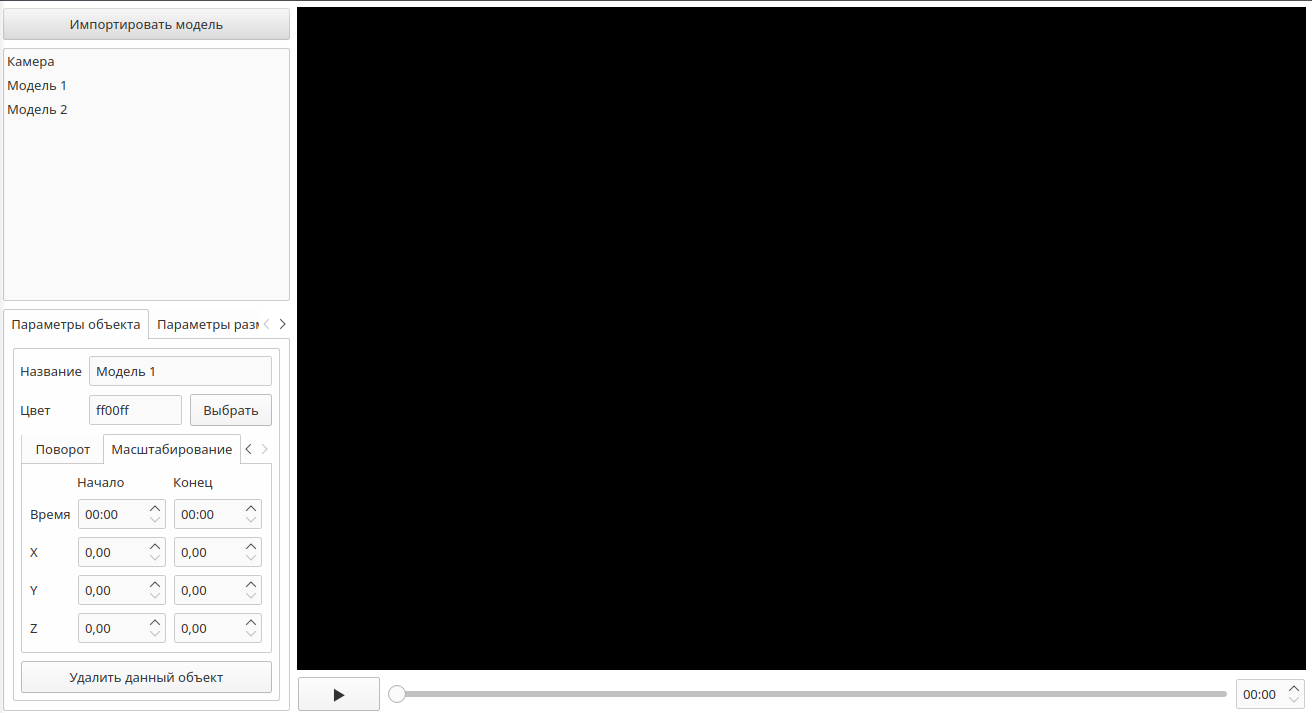
\includegraphics[width=0.9\columnwidth]{img/gui/common.png}
    \caption{Общий вид окна}
    \label{fig:gui_window}
\end{figure}

В правой половине окна расположены предпросмотр сцены и временная шкала. В левой половине список объектов сцены и параметры в виде вкладок. Все вкладки параметров представлены на рисунке \ref{fig:gui_tabs}

\begin{figure}[h]
    \centering
    \begin{minipage}[h]{0.32\linewidth}
        \center{
            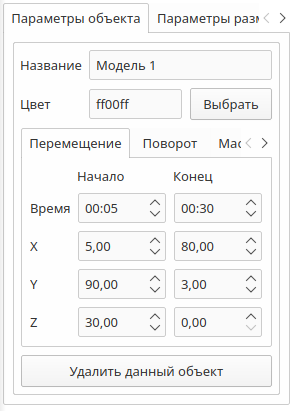
\includegraphics[width=\linewidth]{img/gui/tab1.png} \\ а)
            }
    \end{minipage}
    \hfill\begin{minipage}[h]{0.32\linewidth}
        \center{
            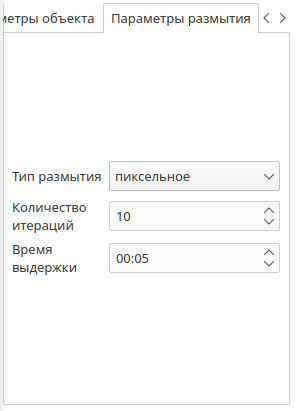
\includegraphics[width=\linewidth]{img/gui/tab2.png} \\ б)
            }
    \end{minipage}
    \hfill
    \begin{minipage}[h]{0.32\linewidth}
        \center{
            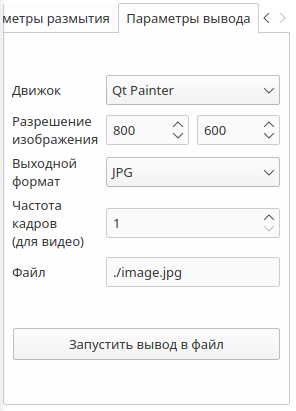
\includegraphics[width=\linewidth]{img/gui/tab3.png} \\ в)
            }
    \end{minipage}
    \caption{Вкладка параметров \\
    а) сцены объекта 
    б) размытия движения
    в) вывода в файл}
    \label{fig:gui_tabs}
\end{figure}

Для изменения параметров определенного объекта пользователю необходимо выбрать нужный объект из списка объектов и внести изменения во вкладке параметров объекта. Также возможно внести изменения в параметры размытия и вывода. 

%%% Local Variables:
%%% mode: latex
%%% TeX-master: "rpz"
%%% End:
